\documentclass[11pt]{article}

\usepackage[margin=1in]{geometry}
\usepackage{amsmath, amssymb}
\usepackage{graphicx}
\usepackage{booktabs}
\usepackage{array}
\usepackage{hyperref}
\usepackage{xcolor}
\usepackage[most]{tcolorbox}
\usepackage{float}
\usepackage{enumitem}
\usepackage{caption}
\usepackage{subcaption}
\usepackage{tikz}
\usetikzlibrary{positioning,arrows.meta}

\hypersetup{colorlinks=true, linkcolor=blue, citecolor=blue, urlcolor=blue}
\graphicspath{{./}{figures/}}

\definecolor{paperbg}{RGB}{244,238,255}
\definecolor{paperframe}{RGB}{103,71,170}
\definecolor{databg}{RGB}{232,248,239}
\definecolor{dataframe}{RGB}{31,122,65}
\definecolor{archbg}{RGB}{231,243,255}
\definecolor{archframe}{RGB}{23,88,156}
\definecolor{trainbg}{RGB}{255,248,220}
\definecolor{trainframe}{RGB}{176,126,0}
\definecolor{cautionbg}{RGB}{255,239,239}
\definecolor{cautionframe}{RGB}{170,50,50}
\definecolor{graybg}{RGB}{247,247,247}
\definecolor{grayframe}{RGB}{90,90,90}

\newtcolorbox{paperbox}[1]{enhanced, breakable, colback=paperbg, colframe=paperframe, title={#1}, fonttitle=\bfseries, arc=2mm, boxrule=0.9pt, left=2mm, right=2mm, top=1mm, bottom=1mm}
\newtcolorbox{databox}[1]{enhanced, breakable, colback=databg, colframe=dataframe, title={#1}, fonttitle=\bfseries, arc=2mm, boxrule=0.9pt, left=2mm, right=2mm, top=1mm, bottom=1mm}
\newtcolorbox{archbox}[1]{enhanced, breakable, colback=archbg, colframe=archframe, title={#1}, fonttitle=\bfseries, arc=2mm, boxrule=0.9pt, left=2mm, right=2mm, top=1mm, bottom=1mm}
\newtcolorbox{trainbox}[1]{enhanced, breakable, colback=trainbg, colframe=trainframe, title={#1}, fonttitle=\bfseries, arc=2mm, boxrule=0.9pt, left=2mm, right=2mm, top=1mm, bottom=1mm}
\newtcolorbox{cautionbox}[1]{enhanced, breakable, colback=cautionbg, colframe=cautionframe, title={#1}, fonttitle=\bfseries, arc=2mm, boxrule=0.9pt, left=2mm, right=2mm, top=1mm, bottom=1mm}
\newtcolorbox{summarybox}[1]{enhanced, breakable, colback=graybg, colframe=grayframe, title={#1}, fonttitle=\bfseries, arc=2mm, boxrule=0.9pt, left=2mm, right=2mm, top=1mm, bottom=1mm}

\newcommand{\vect}[1]{\mathbf{#1}}
\newcommand{\safefig}[2][]{%
  \IfFileExists{#2}{\includegraphics[#1]{#2}}{%
    \IfFileExists{figures/#2}{\includegraphics[#1]{figures/#2}}{%
      \fbox{\begin{minipage}{0.88\linewidth}\centering Missing figure file: \texttt{#2}\end{minipage}}%
    }%
  }%
}

\title{High-Level Report on LSTM-Based Dynamic System Identification of Actuator Response}
\author{Hussein Zolfaghari}
\date{\today}

\begin{document}
\maketitle

\begin{abstract}
This report presents a high-level LSTM-based dynamic system identification procedure for estimating actuator displacement and Lorentz force from two chirp-excitation experiments. The objective is to learn a discrete-time, data-driven model that captures the nonlinear temporal relationship between coil current and the actuator responses. The approach is guided by Wang's LSTM-based dynamic system identification framework, especially the use of discrete-time input-output history and series-parallel identification, and by Ogunmolu et al.'s use of deep dynamic neural networks for sequential system-identification data with regression-based loss and separated evaluation data.

The implemented model uses a series-parallel LSTM structure. At each prediction step, a recent history of coil current, displacement, and Lorentz force is used to estimate the next displacement and force. Because only two chirp experiments are available, both records are divided into train, validation, and test blocks rather than using one full chirp only for training and the other only for testing. The architecture uses two LSTM layers with 64 hidden units, a 120-sample history window, a nonlinear prediction head, weighted multi-output mean-squared-error loss, and regularization tools such as dropout, weight decay, learning-rate scheduling, gradient clipping, and early stopping. These numerical settings are not copied directly from the papers; they are engineering hyperparameter choices selected for this specific two-chirp actuator dataset.
\end{abstract}

\section{Purpose and Main Idea}
The goal of this work is to identify a dynamic model of the actuator directly from measured data. The model receives recent actuator history and predicts the next-step output. The input signal is coil current $I$, and the outputs are displacement $x$ and Lorentz force $F$.

\begin{summarybox}{Main system-identification task}
The actuator is treated as a nonlinear discrete-time dynamic system. The LSTM learns the mapping
\begin{equation}
\{I(k-119:k),x(k-119:k),F(k-119:k)\}\rightarrow [x(k+1),F(k+1)].
\end{equation}
Therefore, the model is not fitting isolated data points; it is learning how recent actuator history affects the next displacement and force.
\end{summarybox}

\section{Connection to the Reference Papers}
The report uses selected ideas from the two reference papers. It does not reproduce every method in those papers; instead, it translates the relevant theory into the actuator-identification simulation.

\subsection{Connection to Wang's LSTM Dynamic Identification Paper}
Wang presents nonlinear dynamic systems in discrete-time form and discusses LSTM-based system identification using input-output history. The most relevant idea for this simulation is the series-parallel identification structure, where measured output history is used together with input history during training \cite{wang2017}.

\begin{paperbox}{How Wang's idea is used here}
Wang's formulation uses past inputs and past outputs to estimate the dynamic response. In this simulation, the same idea is used with actuator variables:
\begin{equation}
\text{input history: }[I(k),x(k),F(k)], \qquad
\text{target: }[x(k+1),F(k+1)].
\end{equation}
The similarity is the use of discrete-time input-output history and measured output feedback during training. The difference is that this implementation predicts two outputs and does not implement Wang's convex multi-LSTM cluster.
\end{paperbox}

\subsection{Connection to Ogunmolu et al.'s Deep Dynamic Neural Network Paper}
Ogunmolu et al. train deep dynamic neural networks on sequential input-output data and evaluate whether the trained model generalizes to separated data \cite{ogunmolu2016}. Their work supports the idea that recurrent/deep neural structures can be used for nonlinear system identification when the data are sequential.

\begin{paperbox}{How Ogunmolu et al.'s idea is used here}
The actuator data are converted into sequential LSTM windows instead of independent static rows. The model is trained by minimizing a regression loss based on prediction error, and performance is evaluated on validation and test windows that are not used for weight updates. This follows the same high-level training and evaluation trend used in deep dynamic system identification.
\end{paperbox}

\section{Dataset and Data Usage}
The dataset contains two experimental records named \texttt{Chirp\_1} and \texttt{Chirp\_2}. Each record is a time-series experiment of the same actuator under chirp current excitation.

\begin{databox}{Meaning of \texttt{Chirp\_1} and \texttt{Chirp\_2}}
\texttt{Chirp\_1} and \texttt{Chirp\_2} are two experimental runs of the same actuator. In each run, a chirp current is applied and the actuator response is recorded over time. They are not two different outputs. Each record contains the input current and the corresponding displacement and Lorentz force response.
\end{databox}

\subsection{Sampling and LSTM Window Creation}
The raw time-series data are resampled to a common time step of
\begin{equation}
\Delta t = 0.002~\text{s}.
\end{equation}
This makes one discrete step have the same physical meaning in both chirp experiments.

\begin{databox}{How many sample times are used for one prediction?}
The sequence length is 120 samples. Therefore, one LSTM input example contains 120 consecutive sampled time instants, and the target is the next sample:
\begin{equation}
[I(1:120),x(1:120),F(1:120)]\rightarrow[x(121),F(121)].
\end{equation}
Since $\Delta t=0.002$ s, the input history corresponds to
\begin{equation}
120\times0.002 = 0.24~\text{s}.
\end{equation}
This 0.24 s history window is long enough to provide recent actuator memory and phase information, while remaining short enough to keep training cost reasonable for only two chirp experiments.
\end{databox}


\subsection{Train, Validation, and Test Strategy}
The two chirp records are kept as separate experimental time series during preprocessing. The data split is then performed inside each chirp using two levels: a block level for organizing the experiment in time, and a window level for creating LSTM training examples.

\begin{databox}{Two-level data organization used in this simulation}
\textbf{Level 1: block-based splitting.} Each chirp is divided into contiguous blocks of 2500 samples. Since the resampled time step is $\Delta t=0.002$ s, each block represents 5.0 s of actuator response. Each block is split by time into 70\% training, 15\% validation, and 15\% testing. 

\textbf{Level 2: LSTM window creation.} After the train/validation/test portions are defined, 120-sample LSTM windows are created inside each portion. Each 120-sample window is used to predict the next sampled displacement and force.
\end{databox}

\begin{figure}[H]
\centering
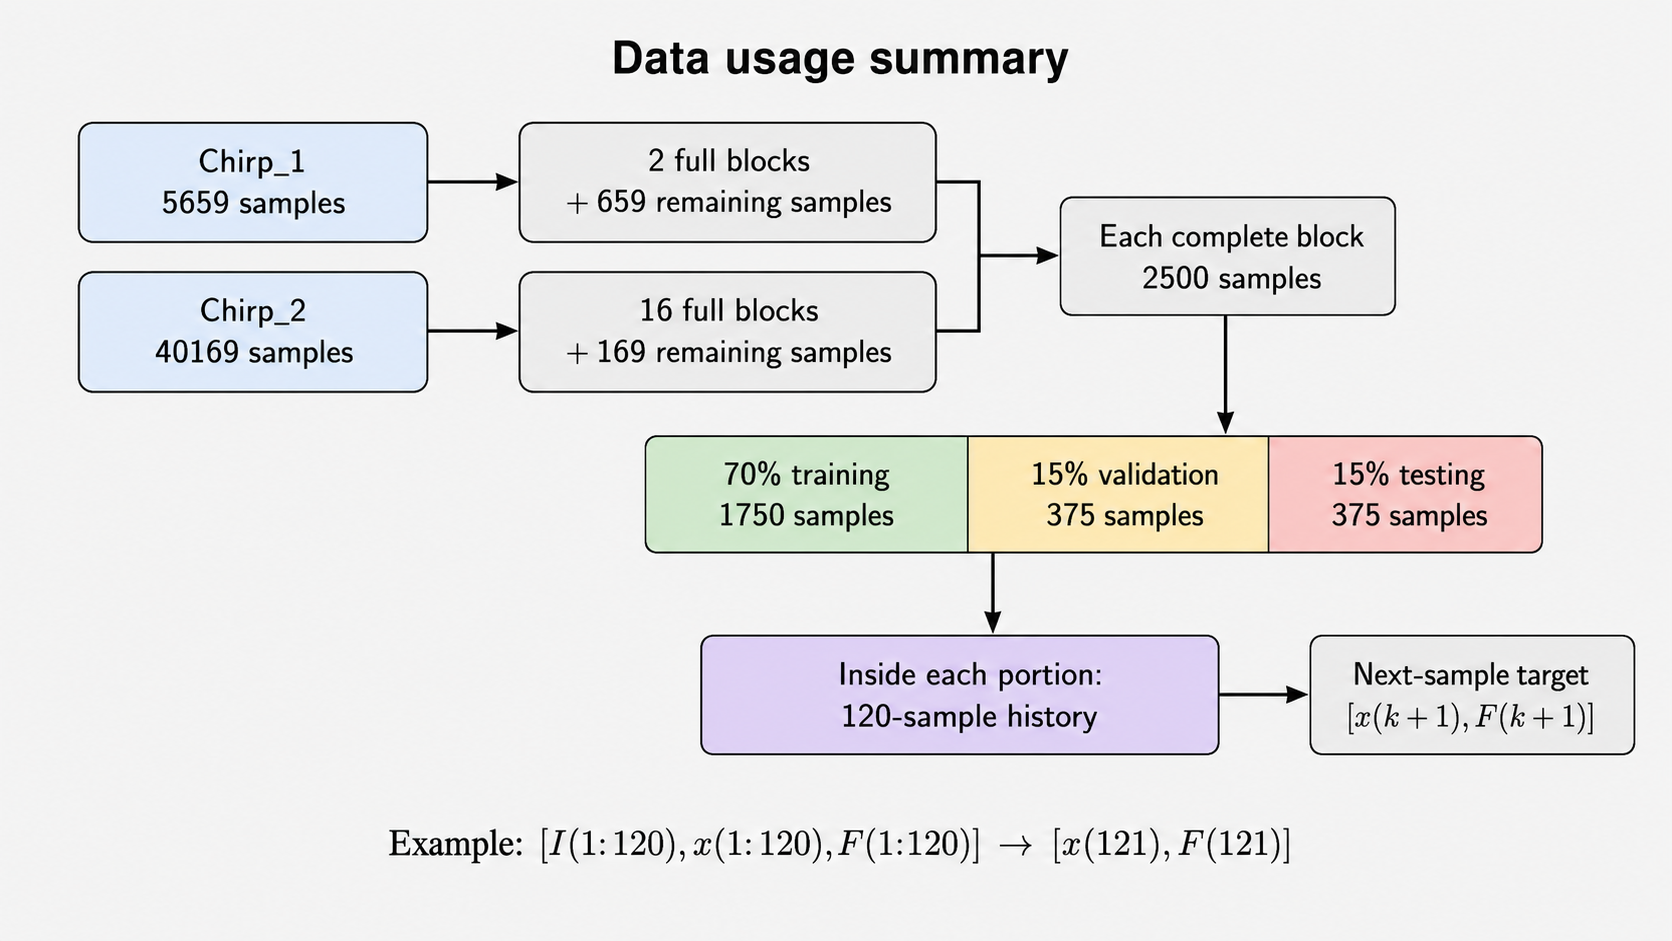
\includegraphics[width=0.98\textwidth]{data_usage_workflow_clean.png}
\caption{Clear data usage workflow. The two chirp experiments are kept as separate time-series records. Each record is divided into 2500-sample time blocks. Each block is split into training, validation, and testing portions. Finally, 120-sample LSTM input windows are created inside each portion to predict the next displacement-force sample.}
\label{fig:block_split}
\end{figure}

\begin{databox}{Numerical interpretation of the data split}
For one 2500-sample block, the split is approximately
\begin{equation}
2500 = 1750\; (\text{training}) + 375\; (\text{validation}) + 375\; (\text{testing}).
\end{equation}
Inside each of these portions, the LSTM examples are formed using a 120-sample history to predict the next sample:
\begin{equation}
1{:}120\rightarrow121,\qquad 2{:}121\rightarrow122,\qquad 3{:}122\rightarrow123,\ldots
\end{equation}
This procedure keeps the experimental records physically meaningful: windows are created within each chirp and within each split portion, rather than across unrelated parts of the dataset.
\end{databox}

\section{Model Architecture}
The implemented model is a multi-output LSTM identifier. In the default series-parallel mode, the input dimension is three:
\begin{equation}
[I(k),x(k),F(k)],
\end{equation}
and the output dimension is two:
\begin{equation}
[\hat{x}(k+1),\hat{F}(k+1)].
\end{equation}

\begin{table}[H]
\centering
\small
\begin{tabular}{p{4cm}p{3cm}p{7cm}}
\toprule
Item & Value & High-level reason \\
\midrule
Input mode & Series-parallel & Uses current plus measured displacement and force history, following Wang's input-output identification idea. \\
Sequence length & 120 samples & Gives 0.24 s of recent actuator history after resampling. \\
LSTM depth & 2 layers & Provides moderate temporal modeling capacity without making the model too deep for two chirp experiments. \\
Hidden units & 64 & Gives enough memory capacity for nonlinear dynamics while limiting overfitting risk. \\
Prediction head & Linear--tanh--dropout--linear & Adds a small nonlinear mapping from the LSTM memory state to the two physical outputs. \\
Output & 2 variables & Predicts next-step displacement and Lorentz force. \\
\bottomrule
\end{tabular}
\caption{High-level architecture summary.}
\label{tab:arch_summary}
\end{table}

\begin{archbox}{Why two LSTM layers?}
Two layers were selected as a balance. One layer may be too limited for nonlinear current-displacement-force dynamics. The first layer extracts temporal features from the measured sequence, and the second layer forms a higher-level dynamic representation. More than two layers would increase the number of trainable parameters and could overfit because only two chirp experiments are available.
\end{archbox}

\begin{archbox}{Why 64 hidden units?}
The hidden size is the dimension of the LSTM memory vector. A small hidden size such as 16 or 32 may not have enough capacity for the nonlinear actuator response. A large hidden size such as 128 or 256 would greatly increase the parameter count and overfitting risk. Therefore, 64 hidden units were selected as a moderate-capacity choice.
\end{archbox}

\begin{summarybox}{Meaning of engineering choices}
An engineering choice means a hyperparameter selected before training for this dataset. The network learns its weights and biases during training, but values such as the number of layers, hidden units, sequence length, learning rate, and dropout are selected by the model designer. The papers justify the modeling direction; the exact numerical settings are chosen for the available actuator data.
\end{summarybox}

\section{Training Method}
The model is trained as a supervised regression problem. Each input window is passed through the LSTM, the prediction head estimates the next displacement and force, and the prediction is compared with the measured target.

\subsection{Loss Function}
A weighted multi-output MSE loss is used:
\begin{equation}
\mathcal{L}=\frac{1}{N}\sum_{j=1}^{N}\left[2.0(\hat{x}_j-x_j)^2+1.0(\hat{F}_j-F_j)^2\right].
\end{equation}
The MSE structure follows the regression-learning idea used in neural-network system identification. The displacement weight is larger because displacement was harder to identify than force in the preliminary runs.

\begin{trainbox}{Why weighted MSE?}
The model predicts two quantities with different physical meanings. Weighted MSE keeps both outputs in the training objective but gives extra attention to displacement, which was the more difficult response to match. This is a practical extension of MSE-based regression to a two-output actuator model.
\end{trainbox}

\subsection{Training Settings}
The main training settings are summarized in Table~\ref{tab:training_summary}.

\begin{table}[H]
\centering
\small
\begin{tabular}{p{4cm}p{3cm}p{7cm}}
\toprule
Setting & Value & Reason \\
\midrule
Optimizer & AdamW & Stable adaptive optimization with weight decay. \\
Learning rate & $5\times10^{-4}$ & Conservative value for stable LSTM training. \\
Dropout & 0.10 & Mild regularization to reduce memorization. \\
Weight decay & $10^{-5}$ & Penalizes overly large weights. \\
Gradient clipping & 1.0 & Prevents large recurrent gradients from destabilizing training. \\
Early stopping & Validation-based & Keeps the model from continuing after validation performance stops improving. \\
\bottomrule
\end{tabular}
\caption{High-level training settings.}
\label{tab:training_summary}
\end{table}

\begin{cautionbox}{How validation MSE should be interpreted}
Validation MSE is usually larger than training MSE because the model directly updates its weights using the training windows. The goal is not to force validation MSE below training MSE. The goal is for validation MSE to decrease, remain stable, and stay reasonably close to training MSE. A large persistent gap would indicate overfitting.
\end{cautionbox}

\section{Simulation Results}
This section presents the main plots generated by the simulation. To keep the report high-level, only representative prediction and error plots are included. Additional test-block plots are saved by the code and can be added if a more detailed appendix is needed.

\subsection{Training and Validation Loss}
\begin{figure}[H]
\centering
\safefig[width=0.85\textwidth]{training_validation_loss_two_chirps_balanced.png}
\caption{Training and validation loss for the two-chirp LSTM training. The important behavior is that the validation loss decreases and remains stable rather than diverging from the training loss.}
\label{fig:loss}
\end{figure}

\subsection{Representative Test Predictions}
\begin{figure}[H]
\centering
\safefig[width=0.92\textwidth]{prediction_Chirp_1_block00_test_two_chirps_balanced.png}
\caption{Representative prediction result for \texttt{Chirp\_1}. The plot compares measured and predicted displacement and Lorentz force on a test block.}
\label{fig:pred_chirp1}
\end{figure}

\begin{figure}[H]
\centering
\safefig[width=0.92\textwidth]{prediction_Chirp_2_block00_test_two_chirps_balanced.png}
\caption{Representative prediction result for \texttt{Chirp\_2}. The model is evaluated on a test block that was not used for weight updates.}
\label{fig:pred_chirp2}
\end{figure}

\subsection{Representative Prediction Errors}
\begin{figure}[H]
\centering
\safefig[width=0.92\textwidth]{error_Chirp_1_block00_test_two_chirps_balanced.png}
\caption{Prediction error for \texttt{Chirp\_1}, calculated as measured output minus predicted output.}
\label{fig:err_chirp1}
\end{figure}

\begin{figure}[H]
\centering
\safefig[width=0.92\textwidth]{error_Chirp_2_block00_test_two_chirps_balanced.png}
\caption{Prediction error for \texttt{Chirp\_2}, calculated as measured output minus predicted output.}
\label{fig:err_chirp2}
\end{figure}

\section{Summary of What Was Implemented}
Table~\ref{tab:traceability} summarizes the most important connection between paper concepts and the implemented simulation.

\begin{table}[H]
\centering
\small
\begin{tabular}{p{4.1cm}p{4.6cm}p{5.8cm}}
\toprule
Paper concept & Implementation in this simulation & Purpose \\
\midrule
Discrete dynamic system \cite{wang2017} & Resampled time-series data indexed by $k$ & Makes the actuator data suitable for next-step prediction. \\
Series-parallel identification \cite{wang2017} & Input vector includes $[I,x,F]$ history & Uses measured output history during training. \\
LSTM memory \cite{wang2017} & Two-layer LSTM model & Learns temporal dependencies in the actuator response. \\
Sequential data learning \cite{ogunmolu2016} & Sliding windows of 120 samples & Trains on time histories instead of isolated rows. \\
MSE regression \cite{ogunmolu2016} & Weighted multi-output MSE & Minimizes displacement and force prediction error. \\
Separated evaluation \cite{ogunmolu2016} & Train/validation/test blocks & Evaluates generalization on unseen windows. \\
\bottomrule
\end{tabular}
\caption{High-level traceability between reference papers and the implemented model.}
\label{tab:traceability}
\end{table}

\section{Conclusion}
An LSTM-based series-parallel dynamic identifier was implemented for actuator displacement and Lorentz-force prediction using two chirp experiments. The model uses recent histories of coil current, displacement, and force to predict the next actuator response. The main theoretical direction comes from LSTM-based dynamic system identification and sequential neural-network system identification. The exact hyperparameters, including two LSTM layers, 64 hidden units, 120-sample sequences, learning rate, and dropout, were selected as dataset-specific engineering choices to balance learning capacity, training stability, and overfitting risk. The results show how the trained model follows the measured actuator response on unseen test windows, while the error plots identify the remaining mismatch.

\begin{cautionbox}{Important limitation}
This work uses only two chirp experiments. Therefore, the model should be viewed as an initial data-driven identifier rather than a fully validated actuator model. A stronger future study should include more experiments with different amplitudes, frequencies, operating conditions, and possibly PRBS or step inputs for better generalization testing.
\end{cautionbox}

\begin{thebibliography}{9}
\bibitem{wang2017}
Y. Wang, ``A New Concept using LSTM Neural Networks for Dynamic System Identification,'' \textit{Proceedings of the American Control Conference}, Seattle, WA, USA, 2017, pp. 5324--5329.

\bibitem{ogunmolu2016}
O. Ogunmolu, X. Gu, S. Jiang, and N. Gans, ``Nonlinear Systems Identification Using Deep Dynamic Neural Networks,'' arXiv:1610.01439, 2016.
\end{thebibliography}

\end{document}
